%%%% ijcai19.tex

\typeout{Probabilistic Robust Multi-Agent Path Finding}


\newcommand{\tuple}[1]{\ensuremath{\left \langle #1 \right \rangle }}

% These are the instructions for authors for IJCAI-19.

\newcommand{\qed}{\hfill\ensuremath{\blacksquare}}
\newcommand{\astar}{A$^*$}
\newcommand{\SAS}{SAS$^+$}
\newcommand{\wastar}{WA$^*$}
\newcommand{\arastar}{ARA$^*$}
\newcommand{\open}{\textsc{Open}}
\newcommand{\closed}{\textsc{Closed}}
\newcommand{\cmfp}{conformant model-free planning}
\newcommand{\eff}{\textit{eff}}
\newcommand{\pre}{\textit{pre}}
\newcommand{\solvable}{\textit{S}}
\newcommand{\plannable}{\textit{P}}
\newcommand{\true}{\textit{T}}
\newcommand{\false}{\textit{$\bot$}}


% This is for the agmin


\documentclass{article}
\pdfpagewidth=8.5in
\pdfpageheight=11in
% The file ijcai19.sty is NOT the same than previous years'
\usepackage{ijcai19}

% Use the postscript times font!
\usepackage{times}
\usepackage{soul}
\usepackage{url}
\usepackage[hidelinks]{hyperref}
\usepackage[utf8]{inputenc}
\usepackage[small]{caption}
\usepackage{graphicx}
\usepackage{amsmath}
\usepackage{booktabs}

\usepackage{float}

%\usepackage{algorithm}
%\usepackage{algorithmic}
\urlstyle{same}

\usepackage{algorithmic}


\usepackage[usenames,dvipsnames]{xcolor}
\usepackage[ruled,vlined,linesnumbered]{algorithm2e}
\usepackage{amsmath}
\usepackage{amsthm}
\usepackage{url}
\usepackage{multirow}

\usepackage{xspace}
\newcommand{\krmapf}{$k$R-MAPF\xspace}
\newcommand{\krcbs}{$k$R-CBS\xspace}
\newcommand{\ikrcbs}{I-$k$R-CBS\xspace}
\newcommand{\prcbs}{$p$R-CBS\xspace}
\newcommand{\iprcbs}{I-$p$R-CBS\xspace}
\newcommand{\prmapf}{$p$R-MAPF\xspace}



%
% Add comments in the text
%
\newboolean{showcomments}
\setboolean{showcomments}{true}
%\setboolean{showcomments}{false}

\ifthenelse{\boolean{showcomments}}
  {\newcommand{\nb}[3]{
  {\color{#2}\small\fbox{\bfseries\sffamily\scriptsize#1}}
  {\color{#2}\sffamily\small$\triangleright~$\textit{\small #3}$~\triangleleft$}
  }
  }
  {\newcommand{\nb}[3]{}
  }

\newcommand\Dor[1]{\nb{\textbf{Dor:}}{red}{#1}}
\newcommand\Roni[1]{\nb{\textbf{Roni:}}{orange}{#1}}
\newcommand\Ariel[1]{\nb{\textbf{Ariel:}}{cyan}{#1}}



\newcommand{\inlinecite}[1]{\citeauthor{#1} \shortcite{#1}}

% the following package is optional:
%\usepackage{latexsym} 

% Following comment is from ijcai97-submit.tex:
% The preparation of these files was supported by Schlumberger Palo Alto
% Research, AT\&T Bell Laboratories, and Morgan Kaufmann Publishers.
% Shirley Jowell, of Morgan Kaufmann Publishers, and Peter F.
% Patel-Schneider, of AT\&T Bell Laboratories collaborated on their
% preparation.

% These instructions can be modified and used in other conferences as long
% as credit to the authors and supporting agencies is retained, this notice
% is not changed, and further modification or reuse is not restricted.
% Neither Shirley Jowell nor Peter F. Patel-Schneider can be listed as
% contacts for providing assistance without their prior permission.

% To use for other conferences, change references to files and the
% conference appropriate and use other authors, contacts, publishers, and
% organizations.
% Also change the deadline and address for returning papers and the length and
% page charge instructions.
% Put where the files are available in the appropriate places.

\title{Probabilistic Robust Multi-Agent Path Finding}

\newcommand{\OPEN} {{\textsc{Open}}}

\newtheorem{definition}{Definition}
\newtheorem{lemma}{Lemma}
\newtheorem{theorem}{Theorem}
\newcommand{\ignore}[1]{}

% Single author syntax
\author{
Dor Atzmon
\and
Ariel Felner\and
Roni Stern
\affiliations
Ben Gurion University of the Negev
\emails
dorat@post.bgu.ac.il,
felner@bgu.ac.il,
sternron@post.bgu.ac.il
}

% Multiple author syntax (remove the single-author syntax above and the \iffalse ... \fi here)
% Check the ijcai19-multiauthor.tex file for detailed instructions
\iffalse
\author{
First Author$^1$
\and
Second Author$^2$\and
Third Author$^{2,3}$\And
Fourth Author$^4$
\affiliations
$^1$First Affiliation\\
$^2$Second Affiliation\\
$^3$Third Affiliation\\
$^4$Fourth Affiliation
\emails
\{first, second\}@example.com,
third@other.example.com,
fourth@example.com
}
\fi

\begin{document}

\maketitle


% -----------------   ABSTRACT    -------------------------
\begin{abstract}

In a multi-agent path-finding (MAPF) problem, the task is to find a plan for moving a set of agents from their initial locations to their goals without collisions.  Following this plan, however, may not be possible due to unexpected events that delay some of the agents. Guaranteeing that collisions will never occur may be impossible. An important task is to find a plan that is very likely to succeed, even though unexpected delays may occur. We propose an algorithm for finding a plan in which the probability that no collisions will occur is at least a given parameter $p$ ($p$-robust plan).
We show that finding an optimal $p$-robust plan is significantly more difficult than finding an optimal standard plan. As a practical solution, we propose a greedy algorithm based on the Conflict-Based Search framework. 
Our experiments show that it finds $p$-robust plans with a cost that is relatively close to the optimal cost of the standard, non-robust plans.
\end{abstract}


% -----------------   Introduction    --------------------------
\section{Introduction}

%\Roni{How about the title ``Probably safe multi-agent pathfinding''? I think it is catchy} [[Vote: 2 to 1]]

The {\em Multi-Agent Path Finding} (MAPF) problem is defined by a graph, $G=(V,E)$ and a set of $n$ agents labeled $a_1 \dots a_n$, where each agent $a_i$ has a start position $s_i \in V$ and a goal position $g_i \in V$. At each time step, an agent can either {\em move} to an adjacent location or {\em wait} in its current location. The task is to find a sequence of move/wait actions for each agent $a_i$ that moves it from $s_i$ to $g_i$ such that agents do not
{\em conflict}, i.e., occupy the same location at the same time. MAPF has practical applications in video games, traffic control, and robotics (see~\cite{felner2017searchBased,MaK17} for surveys on MAPF and related variants and applications). %[[AF: Path is for a single agent. Solution is a valid plan is for the entire set. ]].
In many cases, there is also a requirement to minimize some cumulative cost function such as the sum of costs incurred by all agents before reaching their goals. Solving MAPF optimally is NP-Hard~\cite{DBLP:conf/aaai/YuL13,DBLP:conf/aaai/Surynek10}. Nonetheless, practical optimal algorithms exist, some are even capable of finding optimal plans for more than a hundred  agents~\cite{wagner2015subdimensional,surynek2012towards,yu2013planning,FelnerLB00KK18}.

In practice, unexpected events may delay some of the agents, preventing them from following their pre-determined sequence of move/wait actions. When such an event occurs, the plan of one or more agents should be adjusted to avoid collisions. Such re-planning  may require computing and communication capabilities that can be very costly or even impossible. 
Thus, it is often desirable to generate a {\em robust plan} that can withstand such unexpected events, avoiding the need to re-plan if they occur. This is especially common in safety-critical settings such as air traffic control.

\inlinecite{wagner2017path} proposed an algorithm based on M*~\cite{wagner2015subdimensional} that minimizes the sum-of-costs while keeping the probability of collisions for each individual agent below some threshold.  But, they do not handle the robustness of the plan of the entire set of agents. 


%\Roni{It is not clear what is the difference between robustness of each agent and robustness of the set of %agents. Maybe an example? can we motivate our variant over theirs?}

Recently, a form of robustness called \emph{$k$-robust MAPF} was introduced~\cite{DBLP:conf/socs/AtzmonSFWBZ18}. A $k$-robust plan is robust to $k$ delays per agent, i.e., each agent can be delayed up to $k$ times and the plan guarantees that no collision will occur. This form is especially suitable in cases where the maximum amount of delays is known in advance. However, in many cases an agent may experience more than $k$ delays. Therefore, even a $k$-robust plan may need to be modified during execution. To this end~\cite{ma2017multiAgent} proposed a set of robust online execution policies that avoid collisions during execution . These policies demand online communication and they enforce that the backbone of the plan will be followed. 

In this paper, we explore a novel form of robustness called $p$-robust MAPF (\prmapf{}) designed to produce MAPF plans that can withstand 
unpredictable delays.  In \prmapf{} the task is to find a plan where the probability that no collisions will occur is {\em larger than or equal to} a given threshold $0 \leq p \leq 1$. We show that  finding a minimal-cost $p$-robust plan is computationally harder than standard non-robust plans. %[[AF: we need to strengthen this claim below]]. 
We therefore, propose a greedy CBS-based algorithm that is able to find $p$-robust plans with cost that may not be of minimal cost. Experimental results show that in practice, our algorithm finds $p$-robust plans with cost that is very close to the minimal cost of the standard, non-robust, plan for a range of $p$ values and across several domains. 



% -----------    Definitions and background   ------------------
\section{Definitions and Background}

% MAPF definition.
A solution to a MAPF problem is 
a plan $\pi=\{\pi_1,\ldots \pi_n\}$ 
such that for every $i\in[1,n]$, $\pi_i$ is a sequence of move/wait actions that move agent $a_i$
from $s_i$ to $g_i$. 
$\pi_i(t)$ denotes the location
of $a_i$ after executing the first $t$ move/wait actions in $\pi$ (assuming no delays). Thus, $\pi_i(0)=s_i$ and $\pi_i(|\pi_i|)=g_i$. 

% Conflict definition
\begin{definition}[Conflict]
	A conflict $\tuple{a_i,a_j,t}$ in a plan $\pi$
	occurs iff agents $a_i$ and $a_j$ are located in the same location at time
	step $t$, i.e., when $\pi_i(t)=\pi_j(t)$ (vertex conflict), or when they traverse the same edge when moving from time $t-1$ to $t$, i.e., 
    $(\pi_i(t-1)=\pi_j(t)) \wedge (\pi_i(t)=\pi_j(t-1))$ (edge conflict). 
\end{definition}
We say that $\pi$ is a {\bf valid plan} if it is conflict-free. A MAPF solver
is {\em sound} if it outputs  a valid plan. 

% Conflict-Based Search
\subsection{Conflict-Based Search}
\label{subsec:cbs}
{\em Conflict-based search} (CBS)~\cite{CBSJUR} 
is commonly used MAPF solver that has two levels. The high level of CBS searches the binary {\em constraint
tree} (CT). Each node $N \in CT$ contains: {\bf (1)} a set of constraints
imposed on the agents ($N.constraints$), where a {\em constraint} imposed on
agent $a_i$ is a tuple $\langle a_i,v,t \rangle$, meaning that agent $a_i$ is
prohibited from occupying vertex $v$ at time step $t$; {\bf (2)} a single
solution ($N.\pi$) that is {\em consistent}  with (satisfies) all constraints; and {\bf (3)} the cost of solution $N.\pi$ ($N.cost$), that is, the sum of the path costs of all agents. The root node contains an empty set of constraints. The high level performs a best-first search on the CT, ordering the nodes according to their costs.

{\bf Generating a node in the CT.} Given a node $N$, the low level of CBS finds
a shortest path for each agent that satisfies all constraints in node $N$
imposed on the agent. 

%for example, by using A* with $h$-values that are the
%true distances when ignoring all constraints.

{\bf Expanding a node in the CT.} Once CBS has chosen node $N$ for expansion,
it checks the solution $N.\pi$ for conflicts. If it is conflict-free, then node $N$ is a goal node and CBS returns its solution. Otherwise, CBS {\em splits} node $N$ on one of the conflicts $\langle a_i,a_j,t \rangle$ ($\pi_i(t)=\pi_j(t)=v$) as follows. In any conflict-free solution, at most one of the conflicting agents $a_i$ and $a_j$ can occupy vertex $v$ at time step $t$. Therefore, at least one of the constraints $\langle a_i,v,t \rangle$ or $\langle a_j,v,t \rangle$ must be satisfied. Consequently, CBS {\em splits} node $N$ by generating two children of node $N$, each with a set of constraints that adds one of these two constraints to the set $N.constraints$. 

%%Thus, CBS imposes an additional constraint on only one agent for each child and thus has to re-plan the path %%of only that agent.





% -----------    Multi-Agent Path Finding with Delays   -------------
\section{Multi-Agent Path Finding with Delays}

In the standard MAPF problem we assume deterministic actions execution, i.e., when executing the plan, actions do no fail. However, in reality, when performing move actions one may experience delays during execution. Next, we describe formally such delays and how they can be avoided by creating a robust plan in advance.

% Delay - definition
A \emph{delay} in a plan $\pi$ is defined by a tuple $\tuple{\pi,i,t}$,  
representing that agent $a_i$ did not perform a move action defined for it in $\pi_i$ and instead stayed idle at time $t$ in location $\pi_i(t-1)$.  
Formally, for a plan $\pi$ and 
a delay $D=\tuple{\pi,i,t'}$,
let $D(\pi)$ be the plan 
that is identical to $\pi$ ($\forall j \neq i$, $\pi_j$ remains) except 
for replacing $\pi_i$ with: 
\[\pi_i'(t)=
 \begin{cases} 
      s_i & t=0 \\
      \pi_i(t) & t<t' \\
      \pi_i(t-1) & t \geq t'
   \end{cases}\]
   
   
% Robustness
 \subsection{Robustness}
 
 A plan $\pi$ is \emph{robust} to a delay $D$ if the delayed agent can continue to follow its plan after the delay without causing a collision, i.e., the plan $D(\pi)$ is valid. % A plan $\pi$ is {\em robust} to a delay $D$ if $D(\pi)$ is valid. 
 A plan $\pi$ is {\em robust} to a set of delays $\mathcal{D}$ iff applying any subset of $\mathcal{D}$ to $\pi$ will yield a valid plan, i.e., for every set of delays $\{D_1,\ldots D_T\}\subseteq \mathcal{D}$,  the plan $D_T(D_{T-1}(\ldots D_1(\pi)\ldots )$ is valid. %[[AF: consider to delete]] 
 
 The number of delays may be unlimited. For example, an agent might be dead and might stay idle in its initial location forever. Therefore, for every type of robustness, some form of a bound to the degree of robustness must be given.  One type of robustness is $k$-robust~\cite{DBLP:conf/socs/AtzmonSFWBZ18} and is summarized in the next subsection. In this paper we deal with a new type of robustness -- $p$-robust. In $p$-robust we seek a plan that can withstand unexpected delays with probability {\em greater than or equal to} a given parameter $p$. In this form of robustness we use some of the building blocks from the $k$-robust work. 
 
% \Roni{It seems to me we spend too much on $k$ robust. Why do we need to talk about it more beyond the %paragraph in the introduction?}
% k - Robust MAPF
\subsection{\texorpdfstring{$k$}--Robust MAPF}

$k$-robust MAPF (\krmapf) seeks a  {\em $k$-robust} plan which is a valid plan that is robust to any set of delays that contains at most $k$ delays for each agent. Standard MAPF is a special case of \krmapf{} with $k=0$.  A {\em $k$-delay conflict} $\tuple{a_i,a_j,t}$ in a plan $\pi$ occurs iff there exists $\Delta\in[0,k]$ such that agents $a_i$ and $a_j$ are located in $\pi$ in the same location at time
steps $t$ and $t+\Delta$, respectively, i.e, $\pi_i(t) = \pi_j(t+\Delta)$. A plan is $k$-robust iff it does not contain 
any $k$-delay conflicts. A standard conflict is identical to a $k$-delay conflict with $k=0$. 


% k - Robust CBS
\subsubsection{\texorpdfstring{$k$}--Robust CBS}

{\em $k$-robust CBS} (\krcbs{}) is an adaptation of CBS designed to return optimal (minimal-cost) $k$-robust plans. \krcbs{} differs from standard CBS in how it identifies and resolves conflicts.

{\bf Identifying $k$-delay conflicts.} After the low-level solver returned a
consistent plan for a CT node $N$, \krcbs{} scans $N.\pi$ for $k$-delay
conflicts ($k=0$ for standard CBS). 
%Finding a $k$-delay conflict $\tuple{a_i, a_j, t}$ means that
%$N.\pi_i(t)=N.\pi_j(t+\Delta)$  for $\Delta\in[0,k]$. 
$N$ is a goal CT node iff it has no $k$-delay
conflicts. 

{\bf Resolving conflicts (splitting CT nodes).} Let $N$ be a non-goal node in
the CT selected to be expanded next by \krcbs, and let $\tuple{a_i, a_j, t}$ be
a $k$-delay conflict in $N$. This means that there exist a vertex $v$ and 
$\Delta\in[0,k]$ such that $v=N.\pi_i(t)=N.\pi_j(t+\Delta)$. Note that a
$k$-robust plan does not allow that $a_i$ is at $v$ at time $t$ while $a_j$ is at $v$
at time $t+\Delta$. Similarly, it does not allow that $a_i$ is at $v$ at time $t+\Delta$ while $a_j$ is at $v$ at time $t$. Hence,  every $t_1,t_2\in{[t,t+k]}$ for which $\pi_i(t_1)=\pi_j(t_2)=v$  results in a $k$-delay conflict.  When splitting on a $k$-delay conflict we use {\em range constraints} in the form of $\langle a_i,v,[t,t+k] \rangle$ which prohibit agent $a_i$ from being located at vertex $v$ in any time step $t' \in [t,t+k]$. Therefore, at least one of the following range constraints, $\langle a_i,v,[t,t+k] \rangle$ or $\langle a_j,v,[t,t+k] \rangle$, should be added to the CT and must be satisfied by the low-level solvers. Consequently, \krcbs{} generates two children to $N$, each having one of these constraints. Such range constraints can be safely used to resolve conflicts without losing completeness and optimality~\cite{DBLP:conf/socs/AtzmonSFWBZ18}.


% -----------------   p-Robust MAPF    -----------------------------
\section{\texorpdfstring{$p$}--Robust MAPF}

In some cases, it is possible to estimate the probability that any single delay will occur.  By aggregating the probabilities of multiple delays we can estimate the probability that a given conflict will occur. In such cases, solving all conflicts with the same fixed value $k$ may be less reasonable. For example, a conflict in which agents $a_i$ and $a_j$ are planned to occupy location $v$ at time 1  may have a higher probability to occur than a  conflict in which the agents are planned to occupy $v$ at time 100. Thus, we might prefer solving conflicts based on their probabilities to occur, and not on a fixed $k$. We explore a new form of robustness, $p$-robust, that considers such additional information. In $p$-robust MAPF (\prmapf) given a parameter $p$, ($0 \leq p \leq 1$) we seek a plan that can be executed without any collisions with a probability $\geq p$. 
%[[AF: more motivation with scenarios in real-world]

We next formally define \prmapf{} and then introduce \prcbs, a CBS-based algorithm that solves this problem. 
%setting the same $k$ for all agents may be too restrictive, since it may make more sense to set lower $k$ for conflicts that are less likely to occur (e.g., if they are expected to occur in 100 time steps given no delays) and higher $k$ for conflicts that are more likely to occur (e.g., if they are expected to occur in 5 time steps given no delays).  We explore a new form of robustness, $p$-robust, that considers such additional information. ['[AF: the above few sentences need re-writing]] In $p$-Robust MAPF, given a parameter $p$, we seek a plan that with a probability $\leq p$ can be executed without any collisions.


% Potential conflicts and a conflict occurring
\begin{definition}[Potential Conflict]
A plan $\pi$ has a potential conflict $C=\tuple{a_i,a_j,t}$ iff there exists $\Delta\geq 0$ such that agents $a_i$ and $a_j$ are located in the same location in time steps $t$ and $t+\Delta$, respectively, i.e, when $\pi_i(t) = \pi_j(t+\Delta)$. 
This $\Delta$ is denoted $\Delta(C)$.  
\end{definition}


A potential conflict $C=\tuple{a_i,a_j,t}$ 
is said to {\em have occurred} if 
%during execution   agents $a_i$ and $a_j$ experienced delays that caused $a_i$ to perform the $t^{th}$ action in $\pi_i$  exactly when $a_j$ performs the $(t+\Delta(C))^{th}$ action in $\pi_j$.  This leads to a collision, since $\pi_i(t)=\pi_j(t+\Delta(C))$.  More formally, a potential conflict $C=\tuple{a_i,a_j,t}$ in a plan $\pi$ is said to have \emph{occurred} if 
agent $a_i$ experienced exactly $d_i\geq \Delta(C)$ delays 
before performing the $t^{th}$ action in $\pi_i$, 
and agent $a_j$ experienced exactly $d_i-\Delta(C)$ delays before performing the $t+\Delta(C)$ action in $\pi_j$. This means the agents will collide  since $\pi_i(t)=\pi_j(t+\Delta(C))$ (they will collide at time $t+d_i$).
 

% Our setting, and the likelihood of a potential conflict to occur
The {\em delay probability} is the probability that a given agent will be delayed at a given time step. We assume that such delays are independent 
%\Roni{This is an assumption. In some cases agents' delays may be dependent. So, you should say that this is an assumption that we make in this work.}
, i.e., if one agent is delayed it does not affect the probability that another agent will also be delayed nor the probably that the same agent will be delayed again in a later time step. For simplicity we assume that the delay probability is constant (=$p_d$) across all agents, locations and time steps, although this can be easily generalized. 

In this setting, there is no upper bound $k$ to the number of delays that each agent may experience. Thus, whenever two agents occupy the same location (even in different time steps) they cause a potential conflict and there is some probability that this potential conflict will occur.  Let $P_0(\pi,p_d)$, or $P_0(\pi)$ in short, be the probability that no potential conflict will occur when following plan $\pi$ with a delay probability of $p_d$. 


% p-Robust Plan
\begin{definition}[$p$-Robust Plan]
A plan $\pi$ is $p$-robust if the probability that no potential conflicts will occur is $\geq p$, 
i.e., $P_0(\pi)\geq p$. 
\label{def:likelyRobust}
\end{definition}

A plan $\pi$ is 1-robust if it has no potential conflicts, i.e., the paths induced by $\pi_1,\ldots \pi_n$ are vertex and edge disjoint. Achieving 1-robust plans is a very strong requirement that is rarely needed and may be impossible for many instances where the paths must share some locations.


% Computing the $p$ of a plan is hard for p<1
Verifying that a plan is $p$-robust for some $p<1$ and computing $P_0(\pi)$ are both challenging since the probability that the different potential conflicts will occur is not independent, despite the fact that delays occur independently (according to $p_d$). To see this, consider a plan $\pi$ in which there are two potential conflicts  involving the same pair of agents. %is an agent is a part of two potential conflicts. 
Clearly, these two potential conflicts cannot both occur, 
because when the first of these conflicts occurs the agents collide and cannot continue.  An in-depth discussion on this conflict dependency is provided by \inlinecite{wagner2017path}.


\subsection{Finding Optimal $p$-Robust Solutions}

When standard CBS finds a conflict \tuple{a_i,a_j,t} in node $N$ at location $v$ then that conflict must be avoided. There are three cases: (1) $a_i$ will not be in $v$ at time $t$, i.e., we add the constraint \tuple{a_i,v,t}. (2) $a_j$ will not be in $v$ at time $t$, i.e., we add the constraint \tuple{a_j,v,t}.  (3) both agents will collide at $v$ at time  $t$. Since option 3 is illegal (the conflict must be resolved) CBS splits node $N$ into cases 1 and 2 only, thereby pruning case 3 and its possible descendants and all the solutions in that subtree. This pruning gives CBS its strength.

Now, consider \prmapf. Here we cannot prune case 3 because it may still contain valid $p$-robust plans. This is because the probability for that conflict to actually occur might be small enough that it is still $p$-robust. Thus, if we want to find the minimal-cost solution we must consider case 3 as well. However, splitting a node and generating {\em all} 3 cases does not prune any solution and does not reduce the search space. Therefore, CBS is not helpful for finding optimal solutions for \prmapf{} and we resort to finding any $p$-robust solution fast. However, in our experiments we show that such solutions are of high quality.

In fact, any algorithm that will enumerate {\em all} possible solutions (without pruning) is capable of finding the optimal solution. A more sophisticated pruning method is required to find optimal \prmapf{} plans and this is left for future work.

% ------------------    p -Robust CBS   ------------------------
\section{\texorpdfstring{$p$}--Robust CBS}
 \label{sec:probust-cbs}
 
Next, we describe \prcbs, a CBS-based algorithm designed to return $p$-robust plans.  \prcbs{} is unique in how it handles CT nodes, in how it chooses and resolves conflicts, and in how it orders nodes in the high-level Open list. We next explain the details of \prcbs{} whose pseudo code is given in Algorithm \ref{alg:pRCBS-high}. 


% Handling a CT node
\subsection{Handling a CT Node}

When a CT node $N$ is chosen for expansion (line 5), \prcbs{} scans $N.\pi$ for potential conflicts by simulating the paths and checking for locations occupied by more than one agent (even in different time steps). Then, $N.\pi$ is sent to a binary verifier (line 6) that returns whether the plan is $p$-robust (if $P_0(\pi) \geq p$) or not (if $P_0(\pi) < p$). We discuss implementations of specific verifiers below. If the verifier returns TRUE, then the CT node is declared as goal (lines 7-8). In this case, the search halts and $\pi$ is returned. If   the verifier returns FALSE, it also returns $P_0(\pi)$ as well as a set of probabilities: $P_{First}(C)$, one for each potential conflict $C$\footnote{In the pseudo code the function {\em Verify()} calculates these values in lines 24-25 and they are passed through node $N$.}. $P_{First}(C)$ provides the probability that while executing $\pi$, conflict $C$ will occur first in time among all potential conflicts. That is, $P_{First}(C)$ is the probability that potential conflict $C$ will be the conflict that will cause $\pi$ to fail. Note that the sum of $P_0$ and all $P_{First}$ probabilities equals 1. This is because either the execution of the plan succeeded ($P_0$) or one of the conflicts have occurred and the execution failed (one of the $P_{First}$). 


% Choosing a conflict to resolve
\subsection{Choosing a Conflict to Resolve} 

As explained above, $p$-robust solution may contain many potential conflicts and still be $p$-robust. Thus, while in standard CBS, {\em all} conflicts must be resolved, here we need to resolve a set of conflicts such that the solution will be $p$-robust. There might be many such sets. \prcbs{} chooses to resolve the potential conflict that is associated with the highest probability of occurring (highest $P_{First}(C)$, line 9). This is a greedy approach that has high chances to reach a $p$-robust plan quickly, as it has the highest potential to increase $P_0$ in its children. 


% Resolving a conflict
\subsection{Resolving a Conflict} 

Let $N$ be a non-goal node in the CT selected to be expanded next by \prcbs, and let $C=\tuple{a_i,a_j,t}$ be the chosen potential conflict in $N$. %This means that there is a vertex $v$ and a value $\Delta\in[0,\infty{}]$ such that $v=N.\pi_i(t)=N.\pi_j(t+\Delta)$. 
To resolve $C$, we add the following range constraints
$\tuple{a_i, \pi_i(t), [t, t+\Delta(C)]}$ 
and $\tuple{a_j, \pi_j(t+\Delta(C)), [t, t+\Delta(C)]}$ 
to $a_i$ and $a_j$, respectively (lines 10-13). 
This assures that these agents will not both be at the conflicting location in the time frame $[t,t+\Delta(C)]$. %However, this does not prevent that a new potential conflict will be generated at this location outside this time frame.


% Algorithm - High-level of pR-CBS
\begin{algorithm}[t!]

\begin{footnotesize}
\SetKwBlock{Main}{Main(MAPF problem $instance$)}{end}
\SetKwBlock{GenerateChild}{Generate~Child(Node $N$, Constraint
$C=(a_i,v,[t,t+\Delta])$)}{end}
\SetKwBlock{Verify}{Verify(Node $N$)}{end}

\Main {
%\KwIn{MAPF instance}
    %$R$ $\gets$ new node\\
    Init $R$ with low-level paths for the individual agents\\
    insert $R$ into \OPEN \\
    \While{\OPEN~ not empty}{
    \label{line:p0}
        $N$ $\gets$ best node from \OPEN~ // \emph{highest $P_0$} \\
        \label{line:verifier}
        $\mathit{isGoal} \gets$ Verify($N$)  \\ 
        \label{line:goal}
        \If{$\mathit{isGoal}$}{
        \label{line:return-goal}
            \Return $N.\pi$ // \emph{$N$ is goal}
        }
        \label{line:highest-p-first}
        $C$ $\gets$ get-conflict($N.\mathit{conflicts}$)   // \emph{highest $P_{First}$} \\
        \label{line:delta}
        $\Delta \gets$ get-delta($C$); $v \gets N.\pi(t)$ \\
        \ForEach{agent $a_i$ in $C$}{
        \label{line:generate-child}
            $A \gets \mbox{Generate Child}(N,(a_i,v,[t,t+\Delta]))$\\
            Insert $A$ into \OPEN
        }
    }
}

\GenerateChild {
%\KwIn{Node $N$, Constraint $C=(a_i,s,[t,t+\Delta])$}
        %$A$ $\gets$ new node\\
        $A.constraints \gets N.constraints + (a_i,v,[t,t+\Delta])$\\
        $A.\pi \gets N.\pi$\\
        Update $A.\pi$ by invoking $low~level(a_i)$\\
        $A.cost \gets SIC(A.\pi)$\\
        \Return $A$\\
} \label{GENC}


\Verify {
%\KwIn{Node $N$}
        $\mathit{verification}  \gets$ is-p-robust($N.\pi$) \\
        %\Roni{Why this two steps: first get verification and then ``if'' on it. How about just asking in the ``if'': is-p-robust. If true - your done. If not all the other stuff. }
        \If{$\mathit{verification}$}{
            \Return TRUE // \emph{$P_0 \geq p$}
        }
        $N.P_0 \gets$ get-$P_0$($N.\pi$) \\
        $N.P_{\mathit{First}} \gets$ get-conflicts-probabilities($N.\pi$) \\
        \Return FALSE\\
} \label{VER}

\caption{High-level of \prcbs{}} \label{alg:pRCBS-high}
\end{footnotesize}
\end{algorithm}


% Choosing CT Nodes
\subsection{Choosing CT Nodes}

In \prcbs{} a solution may contain many potential conflicts and still be $p$-robust. Thus, it is not obvious how to choose which CT node to expand. In this paper we focused on finding a $p$-robust plan as fast as possible, relaxing the demand for optimal sum-of-costs. Therefore, we implemented a greedy approach that chooses to expand the node with highest $P_0$ value (line 5). Then,  When a CT node with $P_0\geq p$ is found by a verifier, that node is returned as a goal and the search halts. Another alternative is to choose the node with the minimal sum-of-costs. However even this approach does not guarantee optimality because we cannot prune the case where the conflict still exists (case 3 above).


 %[[AF: need to see whether we want to make a big deal out of this]]


% Figure - pR-CBS Example
\begin{figure}[t]
	\centering
	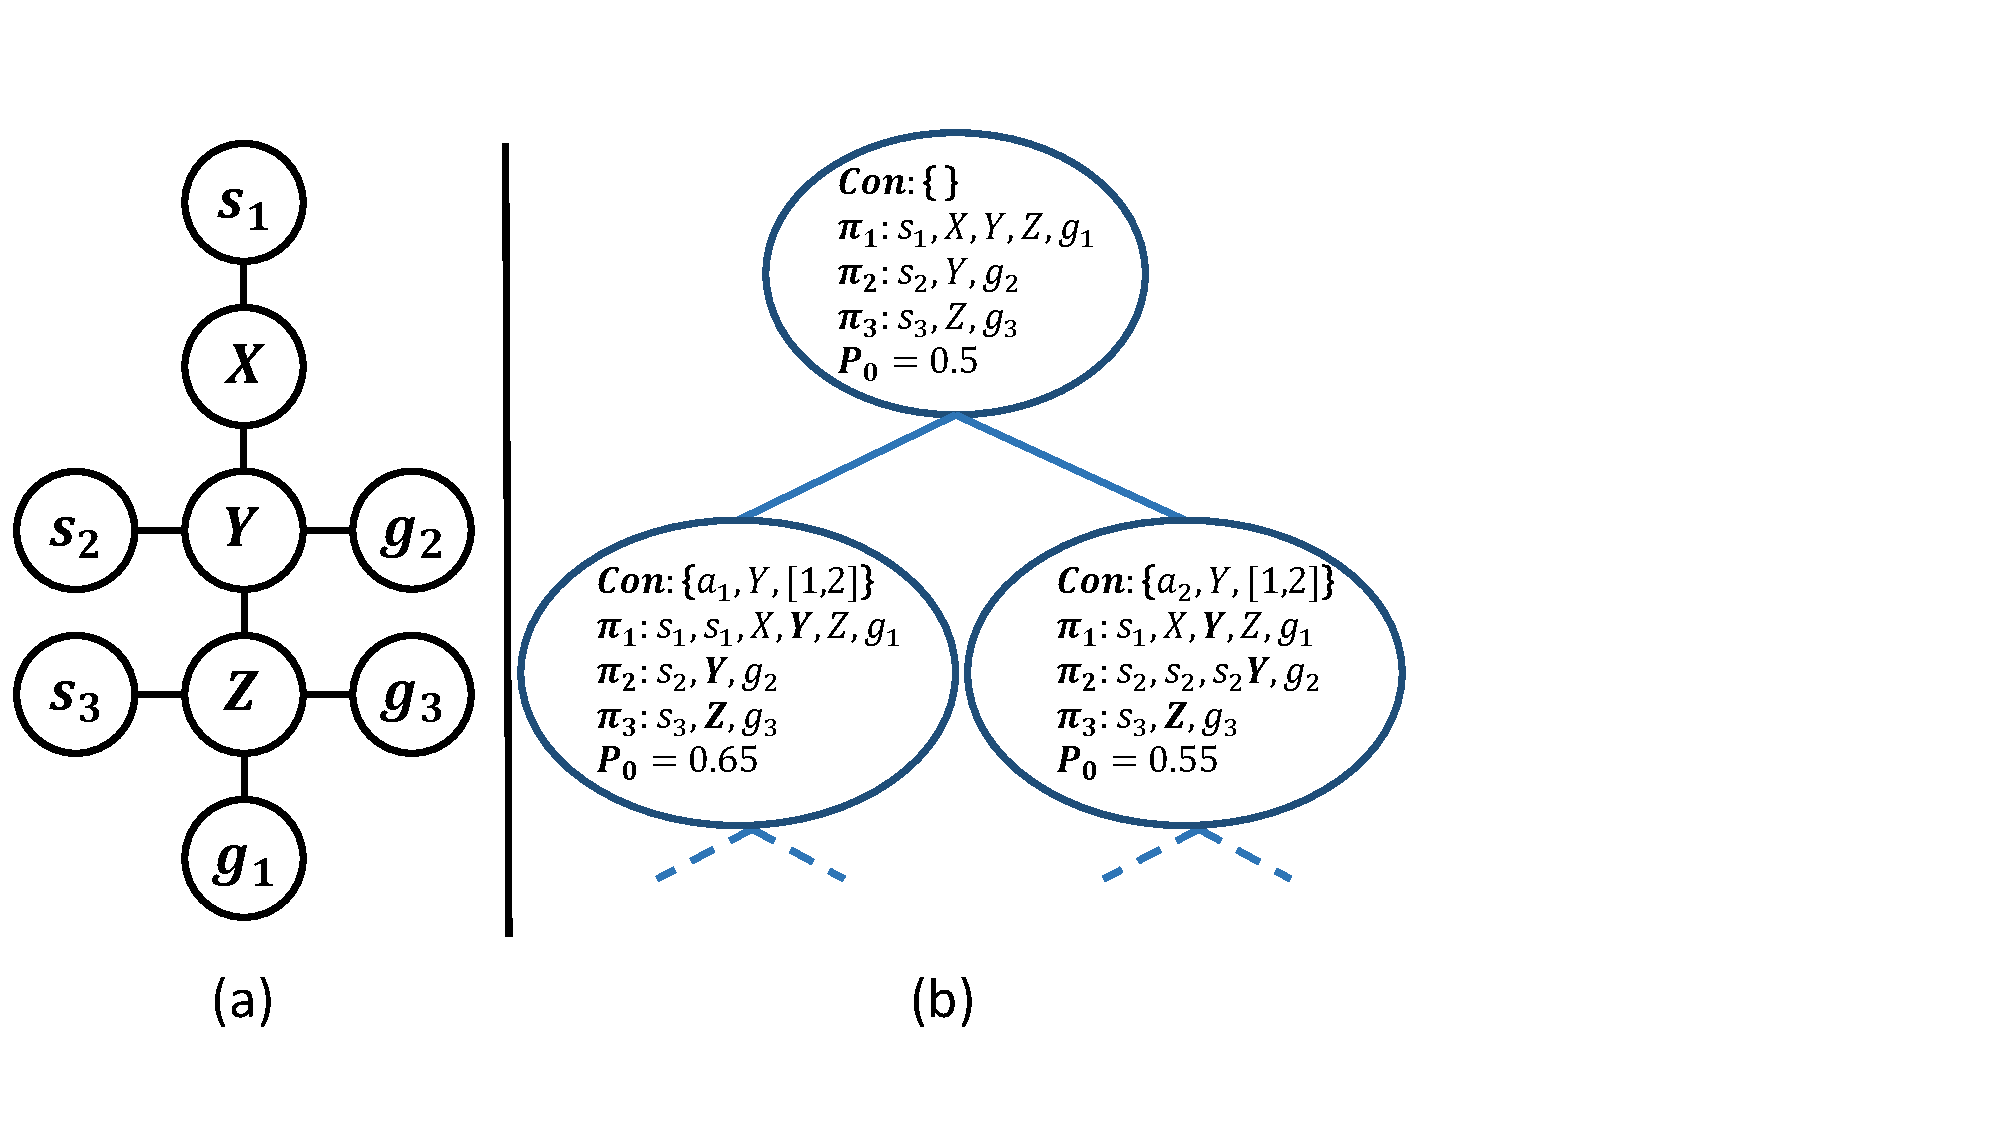
\includegraphics[width=0.85\columnwidth]{Pics/cropped_probust_example.pdf}
	%    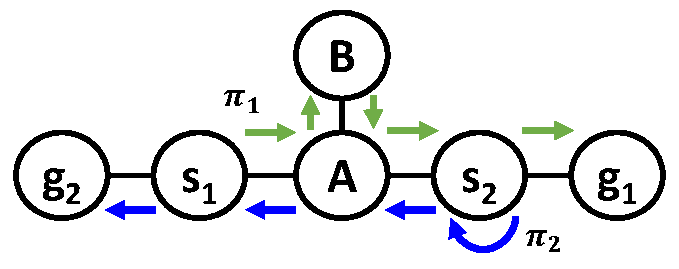
\includegraphics[width=0.9\columnwidth]{lazy-incomplete_cropped.pdf}
	\caption{Example \prcbs{}}
	\vspace{-0.3cm}
	\label{fig:conflicts_example}%\vspace{-0.3cm}
\end{figure}

Figure~\ref{fig:conflicts_example}(a) shows an example of running \prcbs{}. Each of the three agents $a_i$ needs to go from $s_i$ to $g_i$. 
There are two potential conflicts in the initial CT node. $C_Y=\{a_2,a_1, 1\}$ (at location $Y$) where $\Delta(C_Y)=1$ and $C_Z=\{a_3,a_1, 1\}$ (at location $Z$) where $\Delta(C_Z)=2$.
Figure~\ref{fig:conflicts_example}(b) illustrates the corresponding CT. The root of the CT conaints the shortest paths of the three agents. Assume that the verifier returned that $P_{First}(C_Y)=0.3$, $P_{First}(C_Z)=0.2$, and $P_0=0.5$. Meaning that there is a 50\% probability for zero collisions. Assuming $p=0.6$, the verifier returns that the root is not a goal node. We now need to split the CT node by the conflict with the highest $P_{First}$, in our case it is $C_Y$. 
Since $C_Y=\{a_2,a_1, 1\}$ and $\Delta(C_Y)=1$, we resolve $C_Y$ by the set of constraints $\{a_1,Y,[1,2]\}$ and $\{a_2,Y,[1,2]\}$, so that each generates a new CT child node.  After the new paths returned from the low level, we choose the node with the highest $P_0$. This corresponds to the left node (where $a_1$ re-plans). The verifier determines that node as a goal, and \prcbs{} halts. 


\iffalse
Under the assumption that the verifier used by \prcbs is sound, that is, it identifies a plan as being $p$ robust iff it really is $p$ robust, then clearly \prcbs is sound. 

Completeness, however, is a harder 
% ------------  Theoretical Study - TODO  --------------
\section{Theoretical Study}

In this section we theoretically analyze different aspects of \prmapf{} and \prcbs{}.
\Roni{I recommend having this optimal discussion before presenting our solution, as it motivates the fact that our solution is greedy. Then, in this section, only talk about the properties of the new CBS}

%  Adapting CBS for Finding Optimal plans 
%\subsection{Finding Optimal \texorpdfstring{\prmapf{}}. Solutions}


%  Soundness
\subsection{Soundness and Completeness}




\Roni{I agree the discussion below on soundness is trivial. What I wrote above is sufficient and all that's below should be removed, in my opinion.}
A suggested verifier is discussed in Section \ref{sec:stat-verifier}. Here we show that \prcbs{} is sound and complete.

\begin{lemma}[Soundness]
When \prcbs{} returns a plan, the returned plan is a valid solution. 
\end{lemma}
\begin{proof}
Assuming the verifier is sound, if it returns TRUE while \prcbs{} calls to verify a given CT node, than it guarantees that $P_0$ is greater than or equal to $p$. Thus, the probability for no collision of the returned plan ($P_0$) is at least $p$.
\end{proof}
[[AF: Trivial]]


%  Completeness
\subsection{Completeness}

\begin{lemma}[Completeness]
If a valid solution exists, \prcbs{} will return a valid solution. 
\end{lemma}
\begin{proof}
\end{proof}

[[AF: OK. Are we complete??]]

\fi 
% ------------------   Statistical Verifier   ---------------------
\section{Statistical Verifiers}
\label{sec:stat-verifier}

Next, we describe two verifiers that we used (pseudo code is also given in Algorithm~\ref{alg:pRCBS-high}). They verifies statistically whether the robustness of the plan ($P_0$) is {\em greater than or equal to} the desired robustness ($p$). The first verifier performs a fixed number of simulations (Fixed Verifier) while the second verifier dynamically performs simulations (Dynamic Verifier)

%We divide this section into two parts: the initialization of the statistical verifier and the verification %of the statistical verifier.


% Initialization
\subsection{Fixed Verifier}

The fixed verifier is first initialized with the following given parameters: $p$, $p_d$, $s$, and $\alpha$, where $p$ is the desired robustness, $p_d$ is the constant delay probability, $s$ is the number of simulations to be performed, and $1-\alpha$ is the confidence level of the statistical test. Then, a {\em critical value} $c_1$ is calculated by performing a $Z$-test as follows:
\begin{equation}
c_1=p+Z_{1-\alpha} \cdot \sqrt{\frac{(1-p) \cdot p}{s}}
\label{equ:critical}
\end{equation}

$c_1$ is calculated once and used later in every verification to determine whether $P_0 \geq p$ within the confidence level $1-\alpha$.

After \prcbs{} has chosen to expand node $N$ (line 5), it calls the fixed verifier to verify statistically whether $N$ is a goal node (line 21). The verifier executes $s$ simulations of the given plan ($N.\pi$) with delay probability $p_d$. To count collisions during executions we create a table (named $\mathit{occurred}$) that maps a given potential conflict to the number of times it has occurred. We also initialize a parameter: $\mathit{successes}$ that counts the number of executions in which no collision has occurred. During each execution, if a collision has occurred at a potential conflict $C$, the execution halts, and we increment $\mathit{occurred[C]}$ (initialized as $0$). Otherwise, if no collision has occurred, we increment $\mathit{successes}$.

When all $s$ simulations ended, it sets $P_0 \gets \mathit{successes}/s$. If $P_0 > c_1$, it returns TRUE (lines 22-23). Otherwise, it sets $N.P_0 \gets P_0$. For each conflict $C$ it sets $N.P_{First}(C) \gets \mathit{occurred[C]}/{s}$ and it returns FALSE (lines 24-26).

\subsection{Dynamic Verifier}

The main drawback of the fixed verifier is that it uses a fixed number of simulations, denoted $s$. However, in some cases $s$ might not be enough and in other cases $s$ is too high. If $P_0 > c_1$ the verify may return true. This may be possible only if $c_1 < 1$. Therefore, we would like to perform enough simulations that will guarantee that $c_1<1$. This is done dynamically with our dynamic verifier described next, that does not use a fixed number of simulations.  

% Initialization
The minimum number of simulation that guarantees that $c_1<1$ can be derived from Equation \ref{equ:critical}, as follows:
\begin{equation}\label{eq2}
    s \geq \left \lceil {Z_{1-\alpha}}^2 \cdot \frac{p}{1-p} \right \rceil
\end{equation}
For example, for $p=0.95$ and $\alpha=0.05$, we get that $s \geq 73$. So, at least 73 simulations are needed for having the potential of accepting the test. 




% Verification
After initializing $s$ according to Equation~\ref{eq2}, we perform $s$ simulations. We then consider to add more simulations according to the following protocol. We start by testing if $P_0>c_1$. If the test passes, return TRUE. Otherwise, we might be able to perform more simulations until the test will pass. However, the test might always fail and this will lead to an infinite loop.  To overcome this issue, before increasing $s$ and executing one more simulation, we perform another statistical test that checks whether $P_0<c_2$ where $c_2$ is a new critical value which is calculated as follows:
\begin{equation}
c_2=p-Z_{1-\alpha} \cdot \sqrt{\frac{(1-p) \cdot p}{s}}
\label{equ:critical2}
\end{equation}
If the second test passes, return FALSE. Otherwise, increment $s$, execute one more simulation, and perform these two tests again. The verification phase of the dynamic verifier summarized as follows:
\begin{enumerate}
    \item Run $s$ simulations and approximate $P_0$
    \item Calculate $c_1$  (Equation~\ref{equ:critical})
    \item If $P_0>c_1$, return TRUE
    \item Calculate $c_2$ (Equation~\ref{equ:critical2})
    \item If $P_0<c_2$, return FALSE
    \item $s \gets s+1$, run one more simulation, and goto step 2
\end{enumerate}

% ----------------   Experimental Results   ----------------------
\section{Experimental Results}
\label{sec:experiments1}

We experimentally compared the performance of \prcbs{} with different values of robustness $p$, different number of simulations, and different size of domains and with our two verifiers.
In all of the following results $\alpha=0.05$. $P_0$ was calculated based on 50 independent trials of executing the solution. 


% Results - p comparison
\subsection{Different Values of \texorpdfstring{$p$}.}

\begin{table}[t]
\centering
\begin{tabular}{|c|r|r|r|}
\hline
\multicolumn{1}{|l|}{} & \multicolumn{1}{c|}{Cost} & \multicolumn{1}{c|}{Time(ms)} & \multicolumn{1}{c|}{$P_0$} \\ \hline
CBS                    & 38.5                      & 9                         & 0.41                       \\
$p=0.6$                  & 41.7                      & 2,553                     & 0.79                       \\
$p=0.7$                  & 43.3                      & 7,620                     & 0.84                       \\
$p=0.8$                  & 44.9                      & 14,915                    & 0.88                       \\
$p=0.9$                  & 50.1                      & 37,501                    & 0.95                       \\ \hline
\end{tabular}
\caption{Average planning cost, runtime and for CBS and \prcbs{} with different values of $p$,  over 8x8 open grid.}
\label{tab:p-values}
\end{table}

We first compared  standard CBS and \prcbs{} with the fixed verifier for different values of $p$ (0.6, 0.7, 0.8, and 0.9) and $s=40$, on an 8x8 open grid with 8 randomly allocated agents. Table~\ref{tab:p-values} presents the average cost, planning time (in ms), and $P_0$ (out of 50 executions with $p_d=0.2$)  for 60 problem instances.
We can see that larger $p$ increases the cost and time but results in less collisions (higher $P_0$). For example, for $p=0.6$ the cost is 41.7, the time is 2,553ms, and $P_0=0.79$, while for $p=0.9$ the cost is 50.1, the time is 37,501, and $P_0=0.95$. The optimal solver (CBS) achieved the lowest cost (38.5) and the fastest planning time (only 9ms) with a tradeoff that many collisions occurred and only 41\% of the executions were collision-free ($P_0$).


% Results - #Simulations comparison

% Results - DAO map comparison


\begin{table*}[t]
\centering
\resizebox{0.7\textwidth}{!}{
\begin{tabular}{|c|r|r|r|r|r|r|c|c|c|}
\hline
                               & \multicolumn{3}{c|}{Cost}                                                   & \multicolumn{3}{c|}{Time}                                                   & \multicolumn{3}{c|}{$P_0$} \\ \hline
\multicolumn{1}{|l|}{\#Agents} & \multicolumn{1}{c|}{10} & \multicolumn{1}{c|}{20} & \multicolumn{1}{c|}{30} & \multicolumn{1}{c|}{10} & \multicolumn{1}{c|}{20} & \multicolumn{1}{c|}{30} & 10      & 20      & 30     \\ \hline
CBS                            & 1,309.3                 & 2,488.9                 & 3,583.5                 & 268                     & 888                     & 2,377                   & 0.77    & 0.54    & 0.37   \\
p=0.6                          & 1,309.3                 & 2,489.2                 & 3,583.8                 & 8,833                   & 36,051                  & 70,815                  & 0.96    & 0.90    & 0.86   \\
p=0.7                          & 1,309.3                 & 2,489.3                 & 3,583.8                 & 10,063                  & 40,114                  & 79,081                  & 0.98    & 0.90    & 0.88   \\
p=0.8                          & 1,309.4                 & 2,489.4                 & 3,583.8                 & 10,141                  & 53,091                  & 87,206                  & 0.99    & 0.94    & 0.92   \\
p=0.9                          & 1,309.4                 & 2,489.7                 & 3,584.5                 & 10,192                  & 79,299                  & 112,994                 & 0.99    & 0.98    & 0.96   \\ \hline
\end{tabular}}
\caption{Average cost, runtime, and $P_0$ for \prcbs{} with different values of $p$ and number of agents,  over the {\tt brc202d} DAO map.}
\label{tab:dao}
\end{table*}


\iffalse
\begin{table}[t]
\centering
\resizebox{0.97\columnwidth}{!}{
\begin{tabular}{|c|r|r|r|r|r|r|}
\hline
                               & \multicolumn{3}{c|}{Cost}                                                   & \multicolumn{3}{c|}{Time}                                                   \\ \hline
\multicolumn{1}{|l|}{\#Agents} & \multicolumn{1}{c|}{10} & \multicolumn{1}{c|}{20} & \multicolumn{1}{c|}{30} & \multicolumn{1}{c|}{10} & \multicolumn{1}{c|}{20} & \multicolumn{1}{c|}{30} \\ \hline
CBS                            & 1,309.3                 & 2,488.9                 & 3,583.5                 & 268                     & 888                     & 2,377                   \\
p=0.6                          & 1,309.3                 & 2,489.2                 & 3,583.8                 & 8,833                   & 36,051                  & 70,815                  \\
p=0.7                          & 1,309.3                 & 2,489.3                 & 3,583.8                 & 10,063                  & 40,114                  & 79,081                  \\
p=0.8                          & 1,309.4                 & 2,489.4                 & 3,583.8                 & 10,141                  & 53,091                  & 87,206                  \\
p=0.9                          & 1,309.4                 & 2,489.7                 & 3,584.5                 & 10,192                  & 79,299                  & 112,994                 \\ \hline
\end{tabular}}
\caption{Average cost and runtime for \prcbs{} with different values of $p$ and number of agents,  over the {\tt brc202d} DAO map.}
\label{tab:dao}
\end{table}

\begin{table}[]

\end{table}

\begin{figure}[t]
	\centering
	\resizebox{0.8\columnwidth}{!}{
	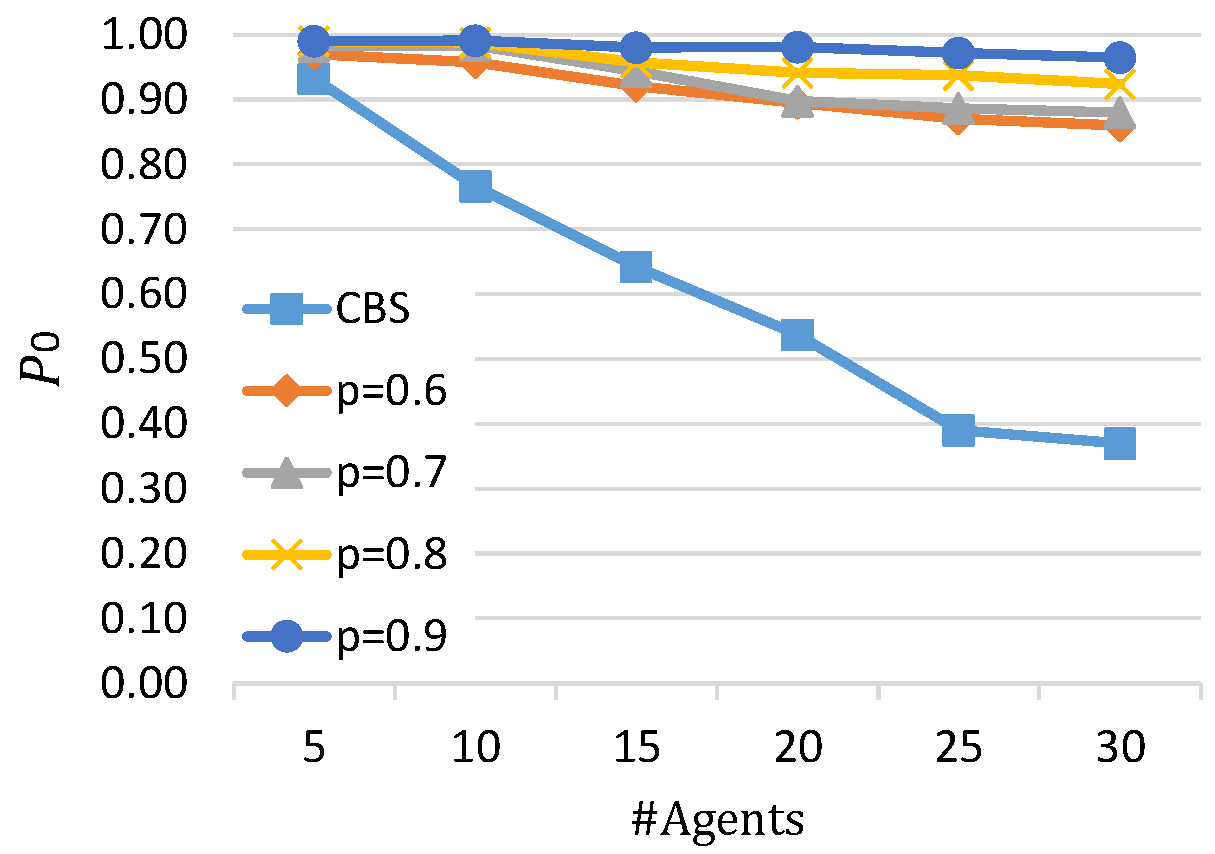
\includegraphics[width=\columnwidth]{Pics/brc202_2.pdf}}
	\caption{$P_0$ for CBS and \prcbs{} over the {\tt brc202d} DAO map.}
	\label{fig:brc_p0}
\end{figure}
\fi

%[[AF: based on space you can delete many of the number examples]]

We also performed experiments on a larger map (called {\tt brc202d}) from the Dragon Age Origin (DAO) video game, which is available in {\tt movingai} repository~\cite{sturtevant2012benchmarks}.
We ran 40 problem instances with 10, 20, and 30 randomly allocated agents. We evaluated CBS and \prcbs{} with $p=0.6,0.7,0.8,$ and $0.9$, $s=40$, and $p_d=0.2$, by measuring the average  cost and planning time. Table~\ref{tab:dao} shows the results of this comparison. Similar to the small domain, increasing $p$ increases also the time. However, unlike the smaller domain, here the cost is very stable for all values of $p$. For example, for 10 agents and $p=0.6$ the cost was 1,309.3 and the time was 8,833ms, while for $p=0.9$ the cost was 1,309.4 and the time was 10,192ms. The reason is that the map is not dense with agents and robust plans can be found of similar costs. In addition, as expected, increasing the number of agents also increases the cost and time. For example, for $p=0.7$ and 10 agents the cost was 1,309.3 and the time was 10,063ms, while for $p=0.7$ and 30 agents the cost was 3,583.8 and the time was 79,081ms.  

Also, we executed every solution 50 times with delay probability ($p_d$) of 0.2, and measured the probability for no collisions ($P_0$).  As expected, all \prcbs{} solvers achieved an higher $P_0$ value than their $p$ values. It is important to show that  $P_0$ for CBS significantly decreases as the number of agents increase. This is because it does not guarantee the robustness and this demonstrates the need for running a $p$-robust solver.  For example, for 5 agents CBS achieved a $P_0$ of 0.93, while for 30 agents CBS achieved a $P_0$ of 0.37, i.e., in only 37\% of the executions no collisions occur.


% -----------   Dynamic statistical verification   -------------
\subsection{Different Number of Simulations}

\begin{table}[t]
\centering
\resizebox{0.97\columnwidth}{!}{
\begin{tabular}{|c|r|r|r|r|}
\hline
\multirow{2}{*}{\#Simulations} & \multicolumn{2}{c|}{$p=0.6$}                             & \multicolumn{2}{c|}{$p=0.8$}                             \\ \cline{2-5} 
                               & \multicolumn{1}{c|}{Time} & \multicolumn{1}{c|}{Expansions} & \multicolumn{1}{c|}{Time} & \multicolumn{1}{c|}{Expansions} \\ \hline
20                             & \textbf{3,066}            & 7.75                         & 13,197                    & 16.70                        \\
40                             & 3,426                     & 7.01                         & \textbf{9,680}            & 10.93                        \\
80                             & 4,324                     & 6.06                         & 14,376                    & 10.67                        \\
160                            & 7,112                     & 5.93                         & 19,848                    & 9.17                         \\
320                            & 12,682                    & 5.75                         & 29,257                    & 8.55                         \\
640                            & 22,397                    & \textbf{5.63}                & 46,065                    & \textbf{7.57}                \\ \hline
\end{tabular}}
\caption{Average runtime, and HL expansions for \prcbs{} with different number of simulation, on a 32x32 grid with 20\% obstacles.}
\label{tab:simulations}
\end{table}
%\roni{Double check please: why is the HL expanded of this one different? i just ran more instances}


Next, we checked the impact of the number of simulations on the average planning time and high-level expansions. We created 60 random problems on a 32x32 grid with 20\% obstacles, and with 10 agents. Table \ref{tab:simulations} shows the average planning time and high-level expansions for \prcbs{} with robustness of $p=0.6$ and $p=0.8$, and delay probability of $p_d=0.2$. 

As can be seen, when $p=0.6$, \prcbs{} with 20 simulations was the fastest (line 1, 3,066ms) and  \prcbs{} with 640 simulations was the slowest (line 6, 22,397ms). However, when $p=0.8$, \prcbs{} with 40 simulations was the fastest (line 1, 9,680ms) and  \prcbs{} with 640 simulations was the slowest (line 6, 46,065ms). It implies that different number of simulations works better for different $p$ values. For both cases ($p=0.6$ and $p=0.8$) the number of high-level expansions decreases as the number of simulations increases. For example, for $p=0.8$, \prcbs{} with 40 simulations expanded average of 16.70 nodes, while \prcbs{} with 640 simulations expanded average of 7.57 nodes. This is because with more simulations the verifier is more accurate is deciding that a solution is indeed $p$-robust. For $p=0.8$, $s=40$ was best in time. This is because for 20 simulations the statistical test passes only by a robust plan with low probability for collisions (high $P_0$), hence it takes more time and expands more nodes. On the other hand when executing simulations the number of expansions decreases but the planning time increases (after 40 simulations) as a result of the simulating time. Therefore, we can conclude that not executing enough simulations or too many simulations results in higher planning time. This experiment shows how sensible is the choice of $s$ and we next experiment with the dynamic verifier.


% Experimental Results
\subsection{Dynamic Verifier}

\begin{table}[t]
\centering
\resizebox{0.95\columnwidth}{!}{
\begin{tabular}{|c|c|c|c|c|}
\hline
\#Simulations & $p=0.80$ & $p=0.8$5 & $p=0.90$ & $p=0.95$ \\ \hline
20            & \textbf{59}     & 0      & 0      & 0      \\
30            & \textbf{59}     & \textbf{59}     & 0      & 0      \\
40            & 58     & 57     & \textbf{57}     & 0      \\
50            & \textbf{59}     & 57     & 55     & 0      \\
60            & 57     & 55     & 55     & 0      \\
80            & \textbf{59}     & 57     & 54     & 51     \\
160           & 58     & 56     & 52     & 49     \\ 
Dynamic       & \textbf{59}     & \textbf{59}     & \textbf{57}     & \textbf{52}     \\ \hline
\end{tabular}}
\caption{Success rate for \prcbs{} out of 60 instances.}
\label{tab:dynamic}
\end{table}

To explore the impact of the dynamic verifier, we compared it to the the fixed verifier (with a different number of simulations) with $p=0.8,0.85,0.9,$ and $0.95$. 60 instances were generated and we present the number of instances that could be solved within 5 minutes in Table~\ref{tab:dynamic}. As expected, if the number of simulations was too small, the fixed verifier could not solve any instance as a result of the statistic test ($c_1$ was greater than 1). For example, \prcbs{} with $p=0.85$ and 20 simulations did not solve any instance. On the other hand, the dynamic verifier could solve instances for all values of $p$. Moreover, the success rate of the dynamic verifier was at least as the success rate of the fixed verifier that achieved the highest success rate. The quality of solution and running time of the dynamic verifier and the fixed verifier were similar for instances that could be solved by both. The dynamic verifier performs better but it is more complicated. Hence there is a tradeoff.


\iffalse
% ----------------   Related Work   -------------------
\section{Related Work}

[[AF: only mention the very important works below that are directly relevant to \prmapf. Do not even mention the improvements to CBS or just mention them all in one setence. Delete this section and merge the remains to the introduction. Add at most a few lines there.]

Wagner and Choset addressed in prior work a similar MAPF settings where agents move according to known probabilistic dynamics, e.g., getting delayed with some known probability~\cite{wagner2017path}. They proposed an algorithm based on M*~\cite{wagner2015subdimensional} that minimizes the sum-of-costs while keeping the probability of collisions for each agent below some threshold. 
Their setting is similar to our $p$-robust setting, but they modified M* while we work with CBS, which outperforms M* in many cases~\cite{ICBS}. Moreover, our solution keeps the total probability for no collisions above some threshold, while their solution treats each agent separately.

Our form of robust planning is different from 
Nguyen et al.'s form of robust planning~\cite{nguyen2017robustPlanning}. 
They consider planning and not MAPF, and address a setting in which an incomplete model of the domain is available and the task is to find a plan that is likely to succeed despite this uncertainty. 

Our description of CBS is of the basic version of CBS. Several improvements to basic CBS have been introduced throughout the years. In {\em Meta-agent CBS} (MA-CBS)~\cite{CBSJUR} agents with many mutual conflicts are merged into a {\em meta-agent}. Meta-agents are then treated as a joint composite agent by the low-level solver. A $k$-robust version of MA-CBS requires that the low-level solver is also $k$-robust for meta-agents consisting two or more agents. Otherwise, the meta-agent might end up having internal $k$-delay conflict.

{\em Improved CBS} (ICBS)~\cite{ICBS} adds three technical enhancements to CBS.
First, it splits conflicts with high likelihood to increase in the
$f$-cost below the corresponding node. Second, it provides a way to ``bypass'' some conflicts and avoid adding nodes to the CT. Finally, it restarts the search from scratch when merging actions occur in MA-CBS. These improvements apply directly to a $k$-robust MA-CBS solver and no further adjustments need to be done.
\fi


% ---------------   Conclusions and Future work   -----------------
\section{Conclusions and Future work}

%[[AF: have all numbers in the same font size]]


In this paper we studied how to generate multi-agent plans that are robust to unexpected changes. We proposed a new form of robustness: $p$-robust. In $p$-robust MAPF -- $p$ is the probability that zero collisions will occur. This form of robustness is suitable when we have some knowledge about the agents' delay probability. We proposed a greedy CBS-based algorithm for finding a $p$-robust plan with two possible verifiers that have internal tradeoff.

There are many possible lines of future work. 
(1) We can adapt other MAPF solvers, such as the ICTS algorithm~\cite{sharon2013increasing}, to find $p$-robust plans. 
(2) We can integrate $p$-robust plans with execution policies, as suggested by Ma et al.~\shortcite{ma2017multiAgent}. 
(3) A deeper study of the $p$-robust setting is needed to bound and better approximate the real $P_0$ probability instead of the approximate we are currently using. 
(4) Development of efficient optimal solvers will enlarge the set of tools for this problem.

%Future work can develop a way to find an optimal $p$-robust plan, meaning the $p$-robust plan will have the minimal cost from all plans that upholds higher probability than $p$ for zero collisions.
%Future work can adapt them to find $k$-robust plans as well. For example, the ICTS algorithm (\cite{sharon2013increasing}) can be 
%adapted to find $k$-robust plans in a similar manner as A* based solvers, , but its tree pruning heuristic will be more costly, requiring comparison with thelast $k$ time steps. Another direction for future work is to develop MAPF solvers that generate plans that can be followed with probability greater than a parameter (\cite{wagner2017pathPlanning}), and to study more reactive execution policies. 



%\section{Discussion: $p$-Robust MAPF}
%In this section we introduce another new variant of the MAPF problem called: $p$-Robust MAPF. In $p$-Robust MAPF, we say that a plan is $p$-Robust if it does not have any collisions with probability greater than $p$. Unlike in $k$-Robust MAPF, where we seek for a plan in which agents must keep a fixed distance from each other. Here, $p$-Robust MAPF fits to cases where the requested plan will contains zero collisions with high probability. Thus, not all agents must keep a fixed distance from each other. Some agents can keep a larger distance while others can keep a smaller one, depending on the probability that the two agents will collide.



%-----------------------------------------------
%-----------------------------------------------


%% The file named.bst is a bibliography style file for BibTeX 0.99c
\bibliographystyle{aaai}
\bibliography{sam}

\end{document}

